\documentclass[12pt]{article}
\RequirePackage{amsthm,amsmath,amsbsy,amsfonts}
\usepackage{graphicx}
%\usepackage{enumerate}
\usepackage{natbib}
\usepackage{url} % not crucial - just used below for the URL 
\usepackage{placeins}

%\pdfminorversion=4
% NOTE: To produce blinded version, replace "0" with "1" below.
\newcommand{\blind}{0}

% DON'T change margins - should be 1 inch all around.
\addtolength{\oddsidemargin}{-.5in}%
\addtolength{\evensidemargin}{-.5in}%
\addtolength{\textwidth}{1in}%
\addtolength{\textheight}{1.3in}%
\addtolength{\topmargin}{-.8in}%


\begin{document}
\section*{Supplementary Material}	 
	
\begin{figure}[h!]
	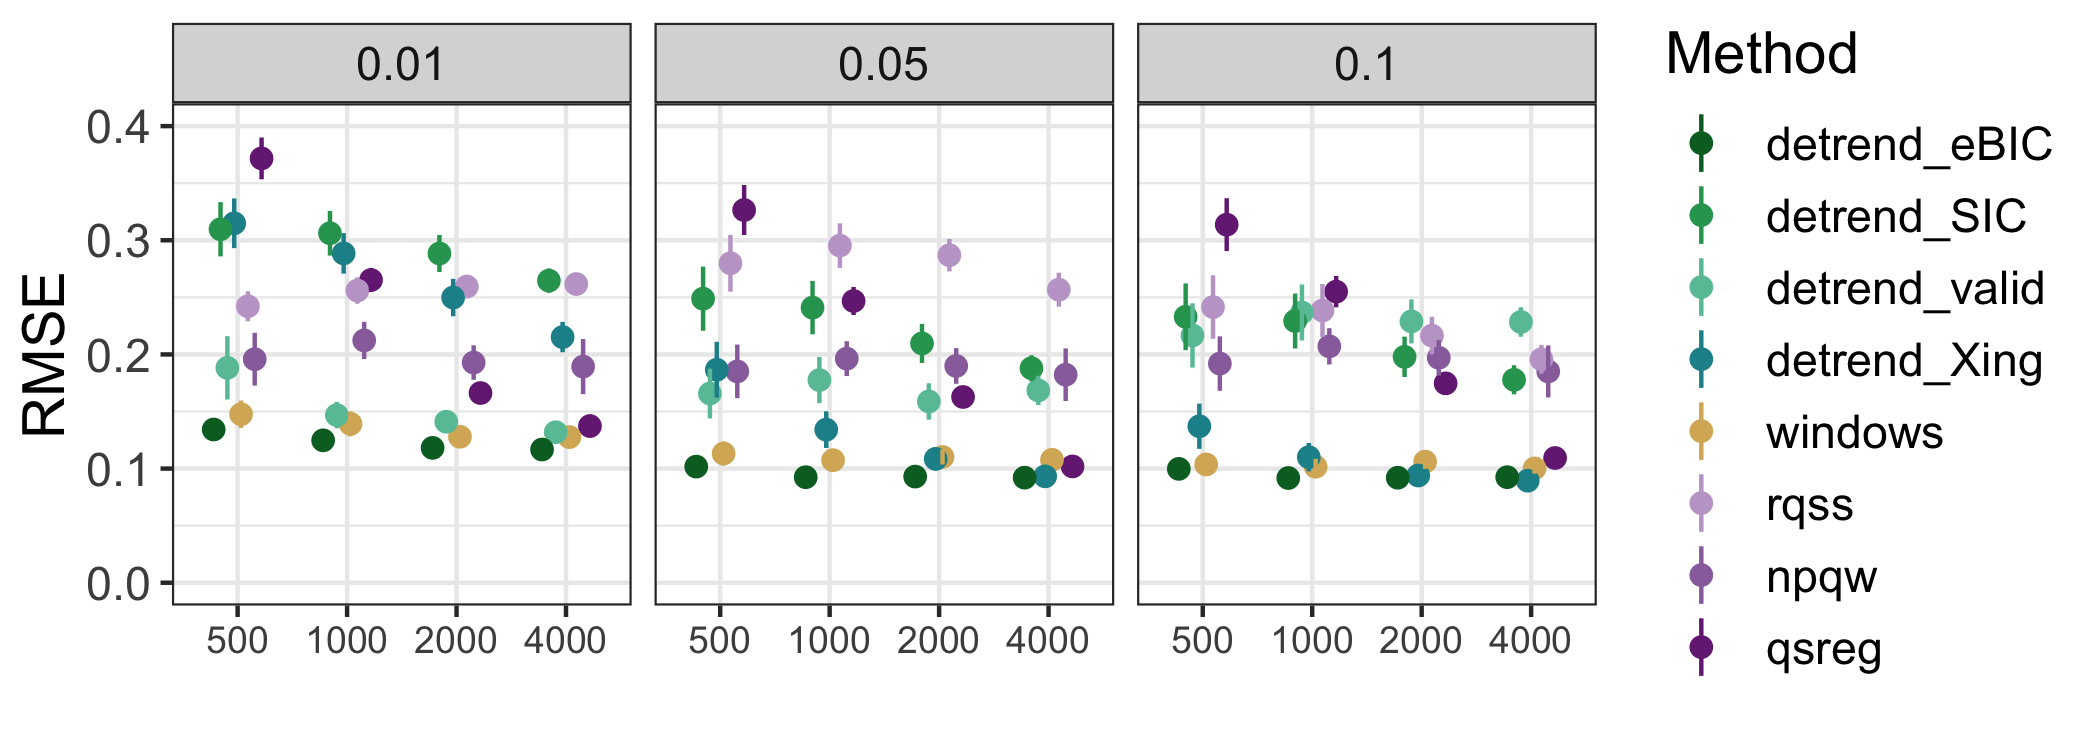
\includegraphics[width = \linewidth]{Figures/peaks_with_windows_mse.png}
	\caption{RMSE by method, quantile, and data size for peaks design. "windows" represents trends fit using 3 windows with an overlap of $n/10$}
	\label{fig:peaks_rmse}
\end{figure}

\begin{figure}[h!]
	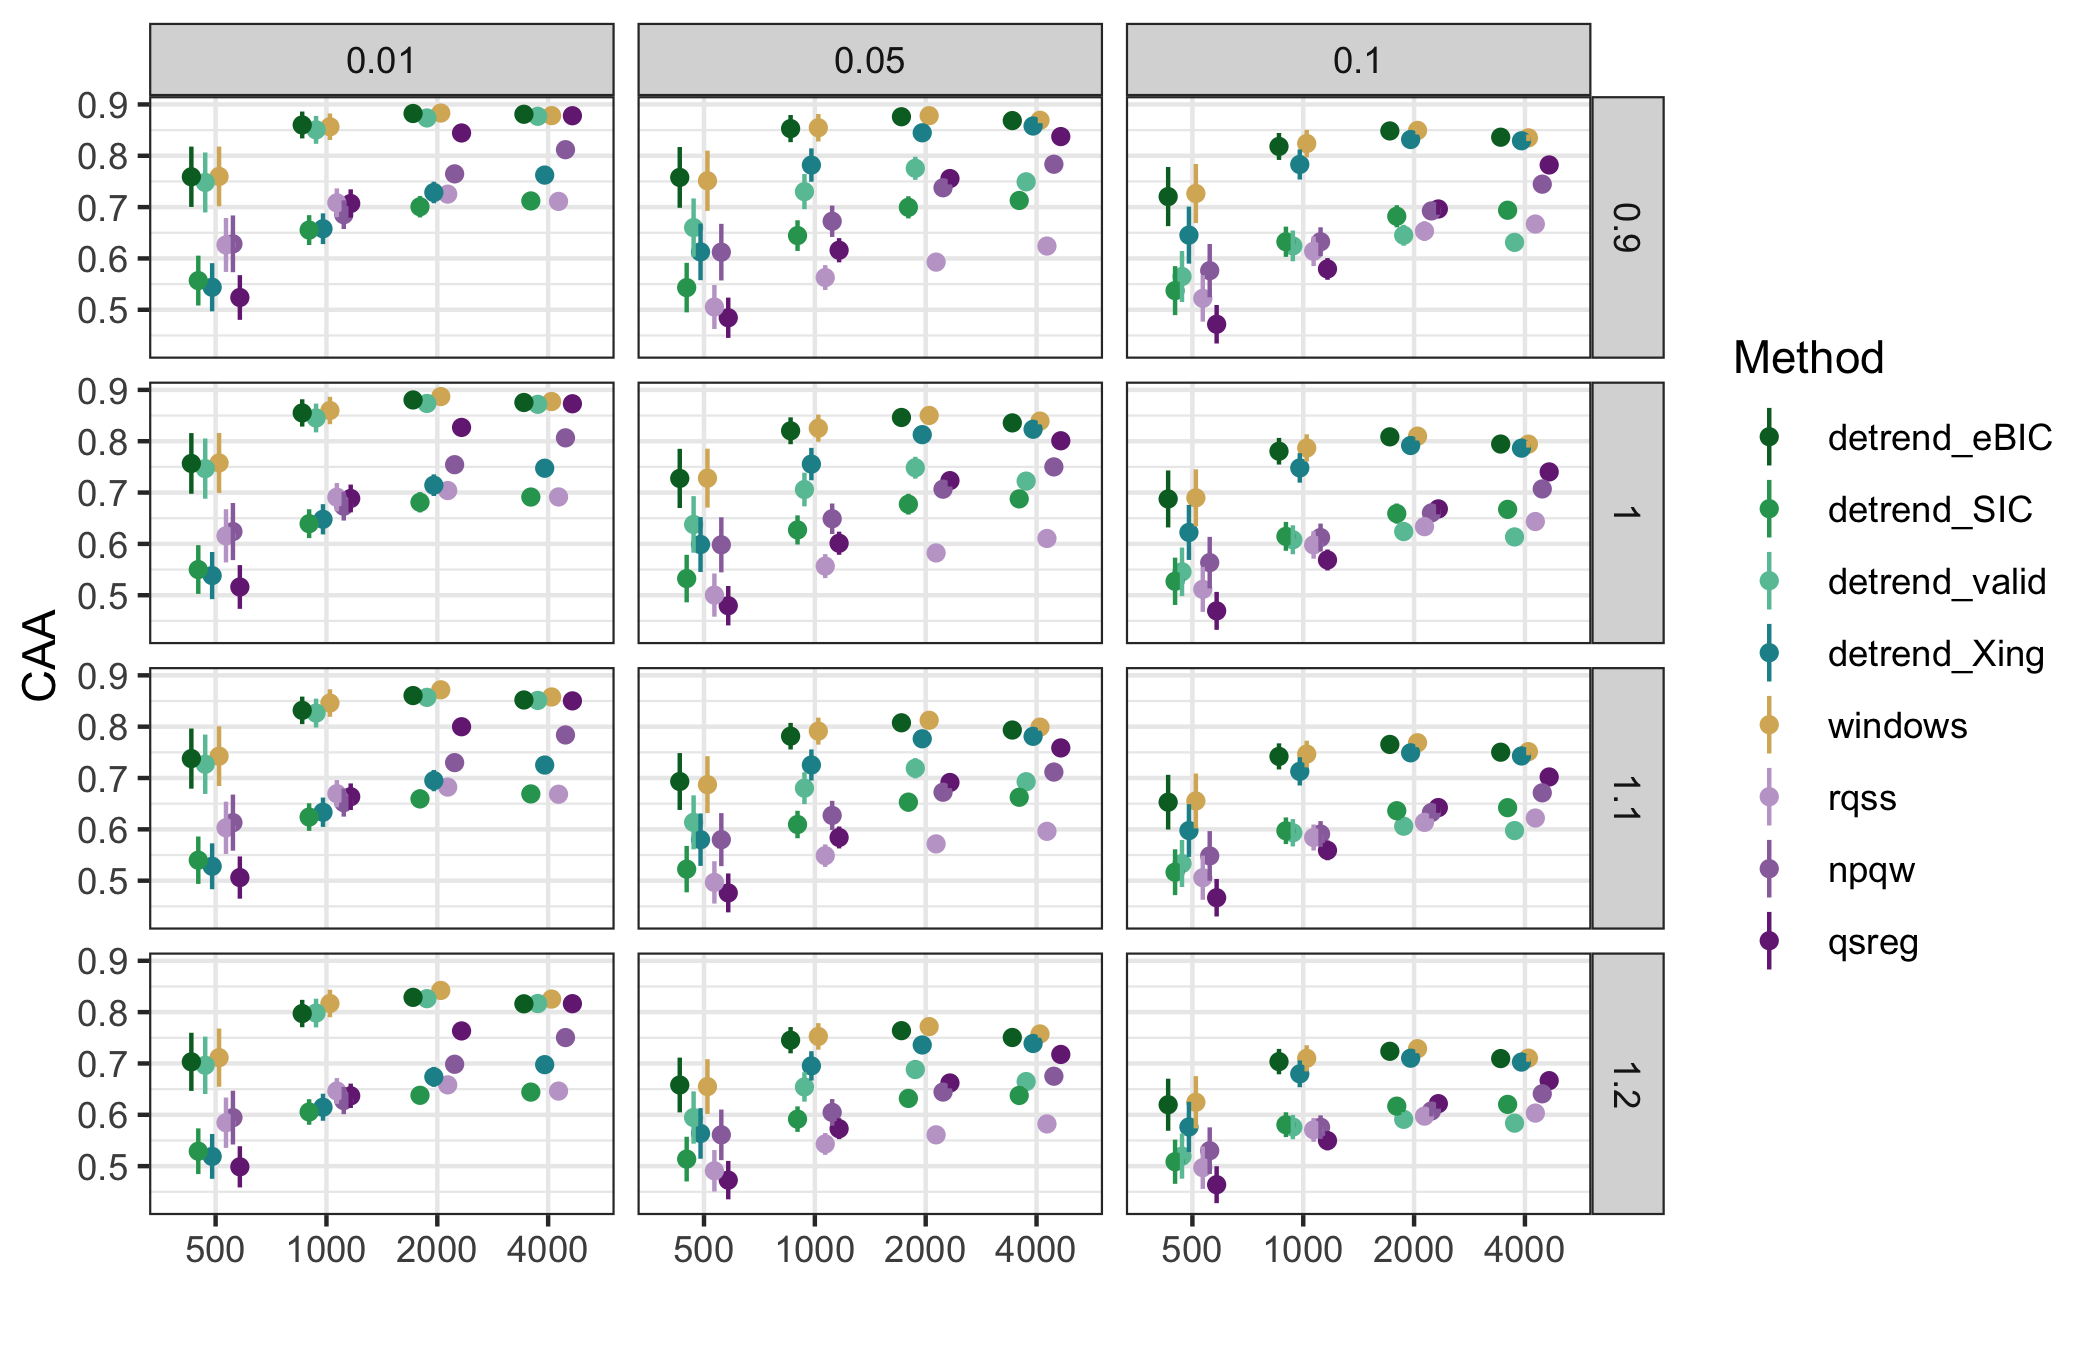
\includegraphics[width = \linewidth]{Figures/peaks_with_windows_CAA.png}
	\caption{Class averaged accuracy by threshold, data size, and method (1 is best 0.5 is worst). "windows" represents trends fit using 3 windows with an overlap of $n/10$}
	\label{fig:CAA}
\end{figure}


\end{document}